%\title{emnlp 2017 instructions}
% File emnlp2017.tex
%

\documentclass[11pt,letterpaper]{article}
\usepackage{emnlp2017}
\usepackage{amsmath}
\usepackage{amssymb}
\usepackage{times}
\usepackage{latexsym}
\usepackage{graphicx}

% Uncomment this line for the final submission:
\emnlpfinalcopy

%  Enter the EMNLP Paper ID here:
\def\emnlppaperid{***}

% To expand the titlebox for more authors, uncomment
% below and set accordingly.
% \addtolength\titlebox{.5in}    

\newcommand\BibTeX{B{\sc ib}\TeX}
% Expectation symbol
\DeclareMathOperator*{\Exp}{\mathbb{E}}

\newcommand{\xxx}[1]{\textbf{\color{red}XXX: #1}}

\title{Speech segmentation with a neural encoder model of working memory}

% Author information can be set in various styles:
% For several authors from the same institution:
\author{Micha Elsner \and Cory Shain \\
        \texttt{melsner0@gmail.com} \and \texttt{shain.3@osu.edu} \\
        Department of Linguistics \\ The Ohio State University,
        Columbus, OH 43210}
% if the names do not fit well on one line use
%         Author 1 \\ {\bf Author 2} \\ ... \\ {\bf Author n} \\
% For authors from different institutions:
% \author{Author 1 \\ Address line \\  ... \\ Address line
%         \And  ... \And
%         Author n \\ Address line \\ ... \\ Address line}
% To start a seperate ``row'' of authors use \AND, as in
% \author{Author 1 \\ Address line \\  ... \\ Address line
%         \AND
%         Author 2 \\ Address line \\ ... \\ Address line \And
%         Author 3 \\ Address line \\ ... \\ Address line}
% If the title and author information does not fit in the area allocated,
% place \setlength\titlebox{<new height>} right after
% at the top, where <new height> can be something larger than 2.25in

\date{}

\begin{document}

\maketitle

\begin{abstract}
We present the first unsupervised LSTM speech segmenter as a cognitive model of the acquisition of words from unsegmented input.
Cognitive biases toward phonological and syntactic predictability in speech are rooted in the limitations of human memory \cite{Baddeley98};
compressed representations are easier to acquire and retain in memory.
To model the biases introduced by these memory limitations, our system uses an LSTM-based encoder-decoder with a small number of hidden units,
then searches for a segmentation that minimizes autoencoding loss.
Linguistically meaningful segments (e.g.\ words) should share regular patterns of features that facilitate decoder performance in comparison to random segmentations,
and we show that our learner discovers these patterns when trained on either phoneme sequences or raw acoustics.
To our knowledge, ours is the first fully unsupervised system to be able to segment both symbolic and acoustic representations of speech.
\end{abstract}


\section{Introduction}

This paper describes a new cognitive model of the acquisition of
word-like units from unsegmented input. The model is intended to
describe the process by which pre-linguistic infants learn their
earliest words, a stage they pass through during the first year of
life \cite{Jusczyk95,Bergelson12}. Our model is based on the standard
memory model of \newcite{Baddeley74} in which the listener encodes
lexical items into phonological working memory, but represents the
entire sentence as a higher-level syntactic structure without
phonological detail. Our model implements this architecture using
encoder-decoder LSTMs with limited memory capacity, then searches for
word segmentations which make it easy to remember the sentence.

Word learning has been extensively studied in previous research, both
with transcribed symbolic input and acoustics. Why attempt yet another
approach? Our model has three main advantages. First, as a cognitive
model, it relates the kinds of learning biases used in previous work
to the wider literature on working memory. Second, its
sequence-to-sequence neural architecture allows it to handle either
one-hot symbolic input or dense vectors of acoustic features. In
contrast, existing models are typically designed for ``clean''
symbolic input, then retrofitted with additional mechanisms to cope
with acoustics. Finally, neural networks have been impressively
successful in supervised language processing domains, yet are still
underused in unsupervised learning. Even systems which do use neural
nets to model lexical acquisition generally require an auxiliary model
for clustering the embeddings, which can make their learning
objectives difficult to understand. Our system uses the
well-understood autoencoder objective to perform the segmentation task
without requiring auxiliary clustering, and thus suggests a new
direction for neural unsupervised learning.

In an experiment conducted on the widely used Brent corpus \cite{Brent99}, our system achieves performance close to that of \newcite{Fleck08}, although subsequent systems outperform ours by a wider margin. 
We show that memory limitations do indeed drive the performance of the system, with smaller LSTM hidden states outperforming larger ones in the development set.

In a follow-up experiment designed to explore the flexibility of our model, we deploy the segmenter on acoustic input: the English portion of the Zerospeech 2015 challenge \cite{Versteegh15}.
Our model outperforms the winning model from that challenge \cite{Rasanen15}, although we underperform more recent unsupervised acoustic segmentation systems \cite{Kamper16,RasanenND}.

To our knowledge, our system is the first unsupervised LSTM speech segmenter, as well as the first unsupervised speech segmenter to succeed on both symbolic and acoustic representations of speech.
Our results are of note for several reasons.
First, they provide modeling support for the claim that memory limitations encourage lexical acquisition.
Second, they show that a general strategy of searching for maximally compressible representations can realistically guide lexical acquisition without explicit reference to perceptual biases \cite[c.f.\ e.g.][]{Rasanen15}, regardless of input representation.
And third, they demonstrate the benefits of our adaptation of neural sequence modeling to unsupervised learning.


\section{Motivations}

We begin with a short overview of previous approaches to the word
learning problem, then explain each of our main contributions in
detail. Many cognitive models of the word learning problem draw on
\newcite{Brent99}, which used a simple unigram model of the lexicon to
discover repeated patterns in phonemically transcribed input. Brent's
model laid the groundwork for later generative models with more
sophisticated prior distributions over word frequencies, co-occurrence
statistics and phonological shapes \cite[among
  others]{Johnson09}. Other modeling architectures for segmentation
have focused on detecting phonological boundaries between words using
transitional probabilities \cite[among others]{Christiansen98} or
inducing words procedurally by ``subtracting'' known word forms from
utterances \cite{Lignos11}.

All these modeling architectures are designed to work with
phonemically transcribed input, and require some degree of
retrofitting to work with more realistic inputs. In the Bayesian
framework, this typically takes the form of a transducer which
probabilistically transforms ``underlying'' lexical items to
``surface'' acoustics \cite{Lee15} or discrete symbols
\cite{Elsner13}; the same framework is used for morphological
segmentation in \newcite{Cotterell15}. For transition-based models,
the input must be transformed into discrete symbols from which
segment-to-segment probabilities can be extracted; this transformation
requires an externally trained preprocessor (a phone
recognizer). Transition-based models are fairly robust to variation in
the symbols \cite{Rytting07,Rytting08,Daland10,Fleck08} and can be relatively
successful in this framework. Extensions using neural nets
\cite{Christiansen98,Rytting08} are discussed in more detail below
(subsec. \ref{sub-neural}). \newcite{Lignos11} requires the most
complex preprocessing of the input (segmentation into syllables, with
marked lexical stresses); adapting it to noisy input is an open
problem.

\subsection{Working memory and learning biases}

Cognitive models of word segmentation rely on two kinds of learning
biases to structure their inferred lexicons: predictability within
words (often expressed as a prior over phonological forms), and
Zipfian unigram and bigram frequencies of words (a prior over word
distributions). These biases control the entropy of utterances, making
it easy for adult listeners to remember what they hear and reconstruct
any missing parts from context \cite{Piantadosi12}. The biases
correspond to different components in a standard model of working
memory \cite{Baddeley07,Baddeley74}. In this model, listeners can
store the last few items they heard in a \textit{phonological loop},
from which words are transferred into \textit{episodic memory} which
represents them at a syntactic/semantic level.


%CS: is this par necessary?
%% Evidence for the phonological loop comes from studies of second
%% language learning. Forcing subjects to articulate a known word like
%% ``the'' (thus occupying their phonological memory) prevents them from
%% remembering foreign-language words, but does not prevent them from
%% learning new associations for known, native-language words. This
%% suggests a dissociation between phonological and semantic memory,
%% which explains why subjects have a greater capacity to recall
%% connected sentences than strings of random words or syllables:
%% Sentences are encoded using episodic memory rather than at the
%% phonological level. When subjects make errors in reconstructing
%% sentences, they remember which ideas they heard, but not the form in
%% which they were expressed \cite{Bransford71}.

\newcite{Baddeley98} claim that the phonological loop functions in
word \textit{learning} as well as processing by proficient listeners,
aiding in the acquisition of unfamiliar words. They summarize a number
of studies showing that the vocabulary size of typically developing
infants correlates with their ability to remember a sequence of
phonologically plausible non-words, a test of phonological loop
capacity. Children with Specific Language Impairment, meanwhile,
remember non-words poorly, a deficit which may contribute to their
atypically small vocabularies. \newcite{Baddeley98} argue that the
ability to remember an unfamiliar phonological form in the short term
is essential if it is to be transferred to long-term memory as a
datapoint for lexical learning. This account of word learning is one
of a growing number which attempt to unify acquisition and speech
processing in terms of the same real-time, resource-constrained
mechanisms \cite{Apfelbaum16}.

In our model, memorization itself can be viewed as the objective for
early word learning. The model attempts to reconstruct its input from
memory; chunks that are easy to reconstruct (and that make the context
reconstructible) are good candidate words. The working memory model
accounts for the two types of bias normally found in Bayesian
segmenters. Phonological predictability due to consistent word shapes
\cite{Boerschinger14,Johnson09} reduces the load on the phonological
loop.  Predictability between words reduces the load on syntactic
memory. The two memory systems draw on different cognitive resources,
which correspond to different parameters of the model.

\subsection{Input representations}
\label{sub-representations}

As stated above, traditional segmentation models operate on phonemic
transcriptions and must be adapted to cope with phonetic or acoustic
input. For models which infer an explicit lexicon (i.e., those which
do not simply count segment transitions), this takes the form of a mapping
between the data and the space of ``underlying'' latent word
forms.

Learning such a mapping can be problematic. Traditional generative
learning models use parametric distributions over the data--- for
acoustics, Gaussians \cite{Vallabha07,Feldman09} or Gaussian-HMMs
\cite{Lee12,Lee15}. But these are a notoriously poor fit to real speech sounds
\cite{Glass03}.

An example of an alternative approach to representation learning from acoustics is \newcite{Rasanen15}.
They exploit known acoustic indicators of syllable boundaries to infer syllable segments, cluster those segments using expectation-maximization (EM), and then identify multisyllabic words by searching for recurring cluster \textit{n}-grams.
As a result, their system is constrained to propose word boundaries only at proposed syllable boundaries regardless of the representations acquired downstream.
Furthermore, EM is known to find non-optimal solutions for many problems in natural language \cite{Johnson07}.
To the extent that this inhibits their system's ability to exploit information in the acoustic feature space, it might lead to misidentification of recurrent syllable \textit{n}-grams and consequently to segmentation error.

Latent underlying representations can also cause search problems,
since the model must explore all the possible underlying forms which
might map to some utterance on the surface. In a probabilistic system
capable of mapping every word to every possible realization, this
quickly becomes intractable. Many systems use dynamic programming
\cite{Mochihashi09,Neubig10}, sometimes with pruning
\cite{vanGael08}. But these algorithms require Markov models with
small context windows, and in any case can still be slow and prone to
search errors.

Neural nets, on the other hand, learn a non-linear mapping between
input and output. This allows them to model speech more flexibly,
outcompeting Gaussian/HMMs for supervised speech recognition
\cite{Graves13,Hinton12}. Recurrent neural nets also produce hidden
representations differently than HMMs. Rather than use dynamic
programming to search a latent space, they produce a single vector
deterministically at each timestep. Models such as LSTMs
\cite{Hochreiter97} can learn long-distance sequential dependencies in
their input without making inference more expensive.

\subsection{Neural unsupervised learning}
\label{sub-neural}

A few previous papers have used neural networks for word
segmentation. \newcite{Christiansen98}, drawing on older work with
Simple Recurrent Networks \cite{Elman90}, trains a recurrent network as
a language model. Word boundaries are extracted at points where the
network predicts an upcoming utterance boundary; that is, utterance
boundaries are used as distant supervision for the locations of word
boundaries. While effective, this system uses symbolic rather than
acoustic input. Moreover, it may have trouble with word endings which
do not end utterances, such as the endings of function words;
experiments show that infants learn detailed representations of
function words by 13 months \cite{Shi06} and use known words as
``anchors'' for segmentation within utterances \cite{Bortfeld05}.

\newcite{Rytting07} adapts the Christiansen model to variable input by
using the posterior probability distribution from a phone recognizer
as its feature representation. This system was run on natural data;
results for word boundary detection were significantly above chance,
though still much less accurate than results for symbolic input. The
use of utterance boundaries as distant supervision may create problems
for this system similar to those pointed out for Christiansen
above. Moreover, the use of an SRN rather than an LSTM means that the
system is essentially phonotatic; it makes its decisions based on the
previous one or two phones, without the capacity to remember whole
lexical items.

Recent work \cite{Kamper16} has attempted to harness the flexibility
of neural feature extractors within the generative model
framework. This model has a hybrid architecture consisting of a neural
feature extractor, the Correspondence Autoencoder, pretrained using
distant supervision \cite{Kamper15}, and a Bayesian
clustering/segmentation model. The system represents each word by
neurally encoding its frames, then downsampling to obtain a
fixed-dimensional word vector; the clustering model assumes that these
vectors can be modeled with Gaussian clusters. The advantage of this
approach is its ability to exploit the known strengths of both
Bayesian and neural learning systems. The disadvantage is its
indirectness: there is no end-to-end objective to be optimized, and
the system's lexical learning does not inform its phonetic
representations.

Even outside the domain of segmentation, neural networks have been
most successful for supervised problems, and are not widely used for
unsupervised learning of discrete structures (trees, clusters, segment
boundaries). While some researchers have proposed
information-theoretic objectives for learning clusters
\cite{Klapper01}, the most widely used unsupervised objective is the
one used here: autoencoding. Yet autoencoders are rarely used to learn
discrete hidden structures. One exception, \newcite{Socher11}, uses
autencoders to find a latent tree structure for sentiment analysis by
greedily merging adjacent nodes so as to minimize the reconstruction
error.

\newcite{Chung17} describe a model similar to our own which performs a
segmentation task using autoencoders. Both models use multiscale
autoencoding to learn a sequence model with unknown segment
boundaries. The main difference is the different technique used to
deal with the discontinuities caused by switching discrete segment
boundary variables. However, they evaluate their model on downstream
tasks (notably, character language modeling) without evaluating the
segmentations directly.

\section{The Model}

The model uses a basic encoder-decoder architecture now typical in
machine translation \cite{Cho14} and image captioning
\cite{Vinyals15}. In a typical encoder-decoder, the input is fed into
an LSTM sequence model \cite{Hochreiter97} which represents it as a
latent numeric embedding. This embedding is then fed into another
sequence model, which uses it to generate an output sequence. Our
two-level model performs this process in stages, first encoding every
word, character-by-character, and then encoding the word sequence,
vector-by-vector. In an autoencoder, the objective is to make input
and output match; thus, the decoder performs the encoding stages in
reverse. We provide the final encoder hidden state as input to each
decoder unit. To force the system's learned embeddings to be robust to
noise caused by mishearing or misremembering, we use dropout
\cite{Srivastava14} at the input (deleting individual timesteps) and
at the word encoding layer (deleting entire words). This architecture
is illustrated in Figure \ref{fig-arch}.

\begin{figure*}
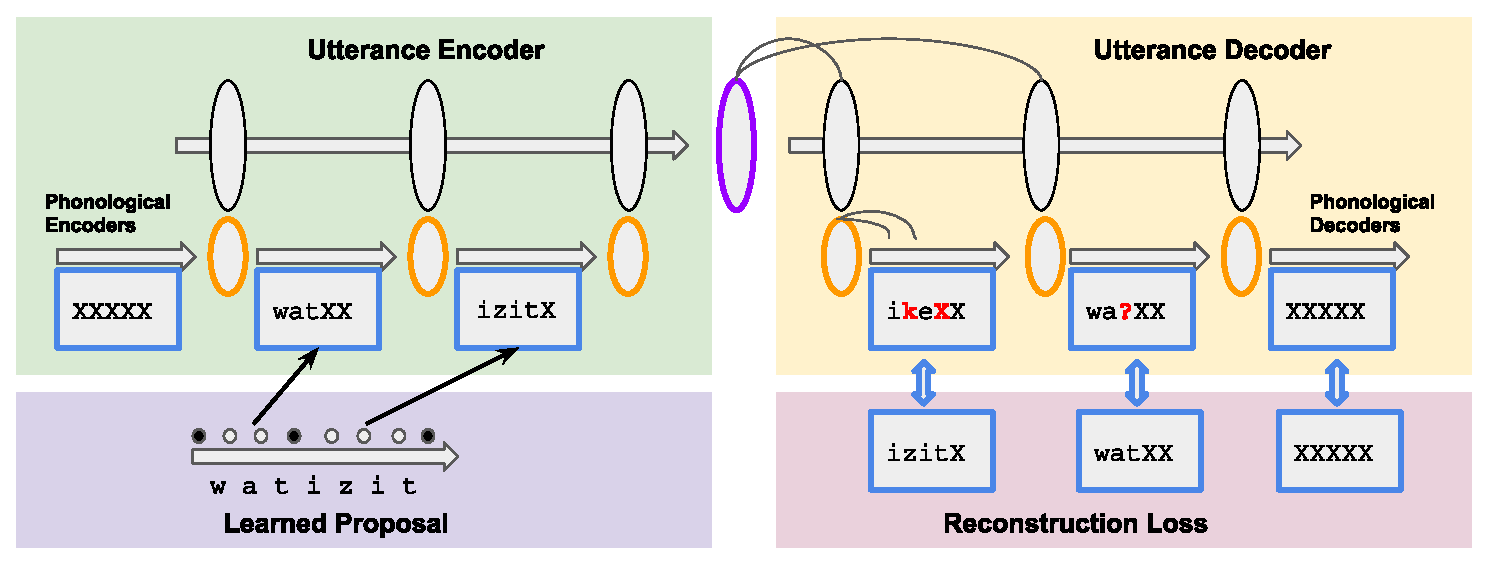
\includegraphics[width=\textwidth]{arch.eps}
\caption{Architecture of the model: top two panels show the
  encoder/decoder, bottom panels show computation of breakpoints and
  resulting loss. Horizontal arrows represent LSTMs.}
\label{fig-arch}
\end{figure*}

The encoder-decoder does not predict segment boundaries directly, but
gives an objective function (reconstruction loss) which can be used to
guide segmentation. Because the segment boundary decisions are hard
(there are no ``partial'' boundaries), the loss function is not
differentiable as a function of the boundary indicators. We use
sampling to estimate the gradient, as in previous work
\cite{Mnih14,Xu15}. Our sampling system works as follows: we
begin with a proposal distribution $P_{seg}$ over sequences of segment
boundaries for the current utterance $x$. We sample $m$ sequences of
boundaries, $B_{1:m}$ from $P_{seg}$. Each boundary sequence splits
the utterance into words. We use the autoencoder network to encode and
decode the words, and obtain the loss (the cross-entropy of the
reconstructed input) for each sequence, $L_{1:m}$.

We can use the cross-entropy to estimate the posterior probability of
the data given a breakpoint sequence (Eq. \ref{eq-post}), assuming a
uniform prior over break positions. We then treat each breakpoint $t$
in the utterance independently: for each one, we use the losses and
the proposal probabilities to compute an importance weight $w_i^t$ for
sample $i$ and position $t$ (Eq. \ref{eq-wt}), then compute the
expected probability of a boundary at that position by summing over
the weighted samples (Eq. \ref{eq-exp}).  Essentially, a breakpoint
will be more likely if it appeared in samples with low reconstruction
loss, especially if it is not encouraged by the current proposal.

\begin{align}
P(x|B_i) &= \frac{P(B_i|x)P(B_i)}{P(x)} \approx \frac{\exp(L_i)}{\sum_j
  \exp(L_j)}
\label{eq-post}\\
w_i^t &= \frac{P(x|B_i)}{P_{seg}^t(B_i^t)}
\label{eq-wt}\\
\Exp[B(t)] &\approx \frac{1}{\sum_i w_i^t} \sum_i w_i^t B_i^t
\label{eq-exp}
\end{align}

We initialize by making random breakpoint proposals (with probability
$.1$ at each position). The random proposal does not search the space
of segmentation boundaries particularly efficiently, so we train a
better proposal using another LSTM. This LSTM simply reads the input
from left to right and predicts a binary output (segment or not) at
each timestep. We update the proposal LSTM by using the
sampling-derived $P_{seg}$ as a training target after each
batch. Thus, the proposal learns to predict segment boundaries that
are likely to result in low reconstruction loss for the main
network. To force the system to explore the space, we smooth the
learned proposal by interpolating it with a uniform distribution:
$P_{seg} = .9 \times P_{LSTM} + .1 \times \frac{1}{2}$.

We control the memory capacity of the system using four tunable
parameters: the number of hidden states at the phonological level
($H_p$) and at the utterance level ($H_u$) and the dropout probability
of mishearing a phonological segment ($D_p$) or a word ($D_u$). We
discuss parameter tuning results below.

The system also has several other parameters which were not tuned
against the evaluation metric. For convenience in GPU training, we
treat all sequences as fixed length, either clipping them or padding
with a dummy symbol. This requires us to set a maximum length for each
word (in characters), and each utterance (in words and characters); we
set these parameters to ensure 99\% coverage of the input (for the
Brent corpus, 7, 10, and 30 respectively).

Clipping creates the possibility of pathological outcomes where the
system deliberately creates extremely long words, exploiting the fact
that the excess characters will be discarded and will not have to be
predicted in the output. We penalize this by subtracting 50 for each
deleted character. Finally, we find that, despite pre-training, the
system may settle into an initial state where the phonological network
simply embeds the characters and the utterance network learns a
character LM. To avoid this, we subtract 10 from the objective for
each one-symbol word. These parameters were tuned only lightly; we
increased the values until the problematic behavior (segmentation of
the entire utterance as one word, or each character as a word) ceased.

We implemented the network in Keras \cite{Keras}, using Adam \cite{Kingma14}
with default settings for optimization. We use mini-batches of 128 and
take 100 samples of potential segment boundaries per sequence. We
perform 10 iterations of pretraining with random boundaries, 10
iterations of boundary induction with random proposals, and 70
iterations of full training with the learned LSTM proposal.

\section{Results}

\subsection{Brent Corpus}

The Brent corpus \cite{Brent99} is a standard benchmark dataset for
segmentation, consisting of 9790 utterances from
\newcite{Bernstein87}, translated into phonemic transcription using
the CMU dictionary. The standard metrics for segmentation are F-score
for word boundary detection (treating each boundary in isolation) and
F-score for word token segmentation (a word is correct only if both
its boundaries are correct and no spurious boundaries
intervene). Although early work on Brent used all 9790 utterances for
both development and test, we use the first 8000 utterances for
parameter tuning. Thus, we present results for the whole corpus (for
comparison with previous work) and clean test results for the last
1790.

%$ python ~/research/neural-segmentation/script/plotTuning.py 
%Best score at wd 0.25 cd 0.5 is 0.829736 at cell 2, 2

We tune the four parameters of our system, $H_p, H_u, D_p$ and $D_u$,
using a grid search (see Figure \ref{fig-gridsearch}). Each subplot
shows a particular dropout setting, $D_p/D_u$; the cells within
represent settings of $H_p$ (rows) and $H_u$ (columns), where darker
cells have higher boundary F-score. Excessive noise decreases scores,
especially high word dropout (right side of the plot). For low levels
of dropout, the best systems tend to have small numbers of hidden
units (dark regions in the lower left); for larger dropout, more
hidden units can be useful. For instance, compare the top left
subplot, with 0 dropout and good performance with $H_p=20, H_u=100$,
to subplot 3,3, with optimal performance at $H_p=80, H_d=200$. In
other words, limiting the system's memory resources is indeed the key
to its performance. The best score occurs at $H_p=80, H_u=400,
D_p=0.5, D_u=0.25$ with a dev boundary F-score of 83\%.
We used these parameters for our final evaluation, along with 100 hidden units in the proposal network.

To further demonstrate that limited memory can bias the network to
learn a low-entropy lexicon, we perform a separate experiment using
the phonological encoder/decoder alone. We create networks with
varying $H_p$ (setting $D_p$ to 0); for each network size, we train
one net on real words from the gold segmentation of Brent, and another
on length-matched pseudowords sampled by randomly segmenting the Brent
corpus. Figure \ref{fig-capacity} shows the reconstruction error rates
as a function of $H_p$. The gap between the green and orange lines
shows the difference in reconstruction error obtained by using real
words rather than pseudowords. For the smallest $H_p$, neither network
does a good job; for the largest, both networks learn the sequences
perfectly. For values in between, however, the lines are relatively
far apart, showing that the real words are easier for the network to
remember.

\begin{figure}
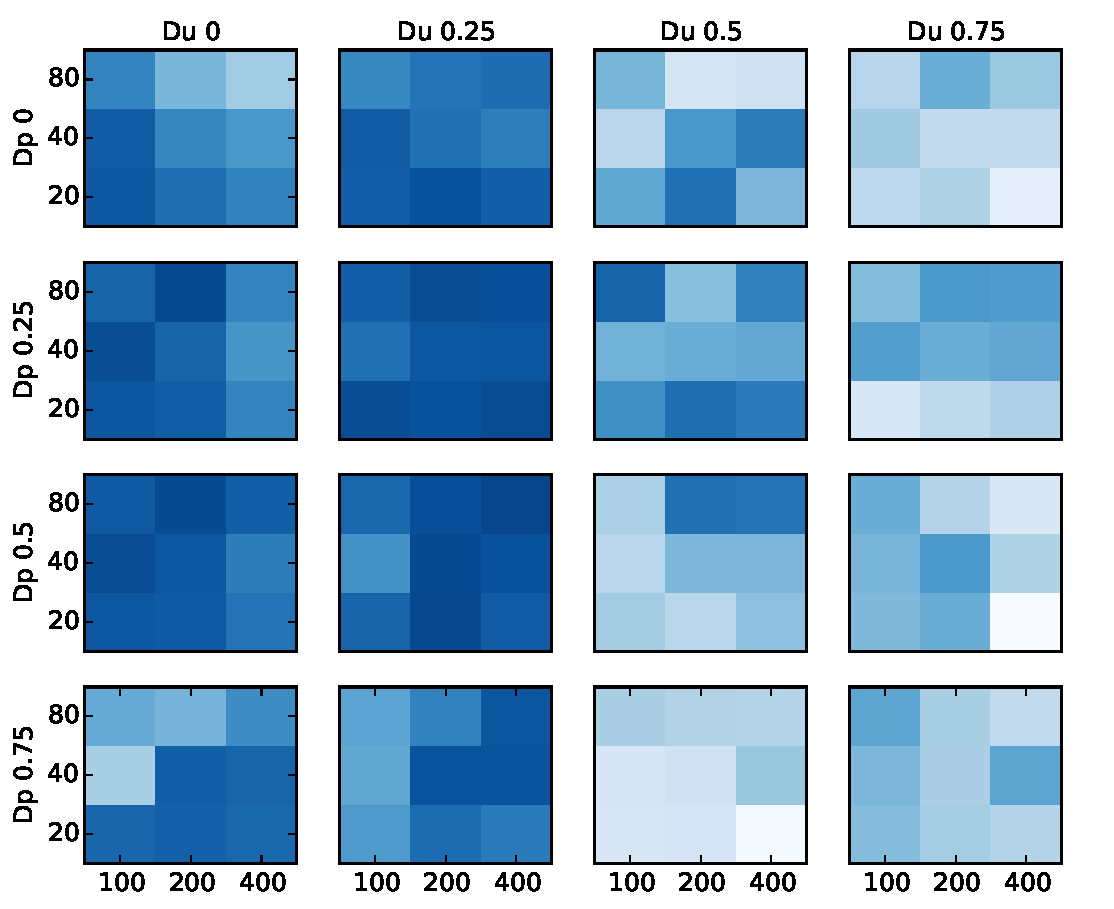
\includegraphics[width=\columnwidth]{heatmap.pdf}
\caption{Tuning results on Brent development. Cell axes represent
  $H_u$ and $H_p$, darker cells have higher scores (best 83\%, worst
  60\%).}
\label{fig-gridsearch}
\end{figure}

\begin{figure}
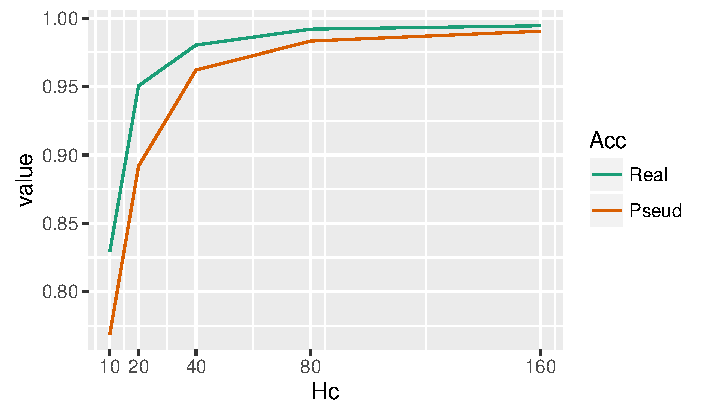
\includegraphics[width=\columnwidth]{capacity.pdf}
\caption{Reconstruction accuracy of the phonological encoder/decoder
  on real words vs. length-matched pseudowords from Brent.}
\label{fig-capacity}
\end{figure}

Our results for Brent, along with selected comparisons, are shown in
Table \ref{tab-results}.\footnote{Comparison system scores are those
  reported in their respective publications, except for
  \newcite{Goldwater09}, which are corrected numbers published with
  their software release. Not all systems report all metrics.} Our
system performs at the lower end of the reported range for Brent
segmenters, scoring 83\% for boundary detection and 72\% for word
detection (comparable to \cite{Fleck08}). (\newcite{Lignos11} scores
93\% boundary F on a different corpus with marked syllable
boundaries.) From a cognitive modeling point of view, it is not clear
what performance we should expect on Brent to model the performance of
a young human infant. Models of early word segmentation are motivated
by studies showing that, by their first birthday, infants can
distinguish many common words from nonwords
\cite{Vihman04,Swingley05}. But this does not imply that they learn
every word they hear, or that they can use their word knowledge to
segment every utterance correctly. Thus, while our result is not
state-of-the-art, it is good enough to conform with the reported
infant results and suggest that our neural architecture is a promising
direction.

%% our test results from logs/w80-u400-s100-wd0.25-c0.5/

\begin{table}
\begin{tabular}{p{2.1cm}cccc}
System & Bd P & Bd R & Bd F & Wd F\\
\hline
Goldwater 09       & 90 & 74 & 87 & 74\\ 
Johnson 09         & - & - & - & 88\\
Berg-Kirkpatrick 10 & - & - & - & 88\\
Fleck 08           & 95 & 74 & 83 & 71\\
\hline
Ours (all) & 81 & 85 & 83 & 72\\
Ours (test) & 81 & 86 & 83 & 72\\
\end{tabular}
\caption{Selected segmentation results on Brent.}
\label{tab-results}
\end{table}

Learning curves for segmentation on the Brent corpus are shown in
Figure \ref{fig-learning-curve}. The first 10 iterations show a
gradual increase in segmentation performance using the random
proposal. Performance increases sharply with the activation of
the learned proposal, then climbs slowly over time. Precision
initially exceeds recall (that is, the system proposes too few
boundaries) but recall climbs over time as the system exploits known
words as ``anchors'' to discover new ones, a pattern consistent with
the infant data \cite{Bortfeld05}.

\begin{figure}
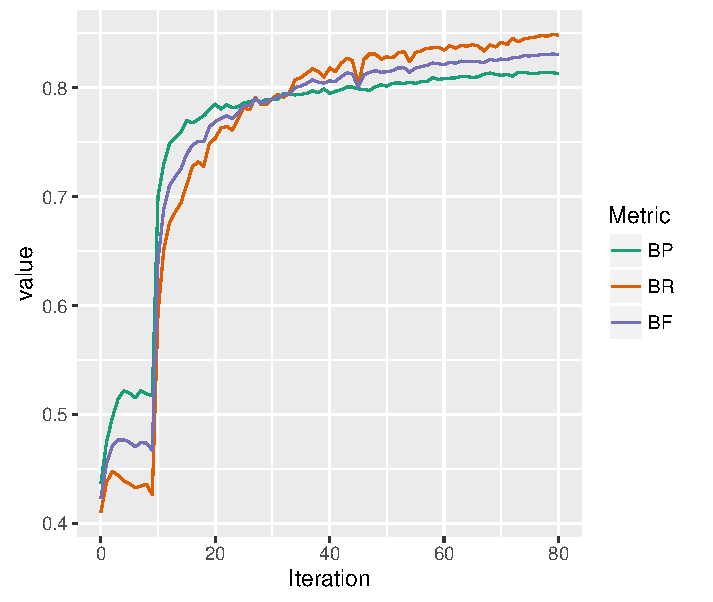
\includegraphics[width=\columnwidth]{learning-curve.pdf}
\caption{Boundary precision, recall, and F1 score by iteration on the
  entire Brent dataset.}
\label{fig-learning-curve}
\end{figure}

\subsection{Zerospeech 2015 acoustic segmentation}

We began by claiming that an advantage of our model was its flexible
architecture that permits dense acoustic features as input (rather
than symbolic phone labels) with little modification.  In this
section, we present preliminary results from a follow-up experiment in
which we tested this claim by deploying our system as an acoustic
segmenter on the English portion of the Zerospeech 2015 challenge
dataset \cite{Versteegh15}.  We preprocess the raw acoustic data by
extracting 25ms 13-dimensional mel frequency cepstral coefficients
with first and second order deltas at a step size of 10ms.  We then
train the network on the resulting sequences of 39-dimensional
frames.

Given that the goal of the experiment was to test the existing architecture on a novel task, we intentionally conducted this experiment with minimal parameter tuning or architectural modification.
However, we made several key changes in response to the unique challenges presented by acoustic input.

First, since we are now reconstructing dense vectors of acoustic
features, we use mean squared error (MSE) instead of categorical
cross-entropy as the autoencoder loss function.  We consequently
rescale our clipping penalty from 50 to 1, a coefficient which seemed
more in balance with the variation in decoder loss produced by MSE.
We also increase our one-letter penalty from 10 to 50, modeling our
strong prior assumption that a 1-frame segment will never correspond
to a word.

Second, in contrast to the phoneme sequences in the Brent corpus
discussed above, utterance boundaries are not observed in acoustic
input.  The input to the two-level autoencoder must be divided into
sequences of utterances, so we imposed utterance boundaries by
iteratively consuming the next discovered word in the time series up
to the maximum utterance length (in frames).  The aforementioned
clipping penalties punish the system for utterances that contain too
many words, preventing it from optimizing its autoencoder loss by
segmenting everywhere.

Third, for our initial proposal distribution we use the speech region
segmentation provided by the Zerospeech challenge, consisting of
speech intervals identified through automatic voice activity detection
(VAD), rather than using the uniform initialization described above
for symbolic mode.  We interpolate the initial distribution with a
uniform prior as described above.

Fourth, we discovered in practice that the assumption of independence
between samples made by the importance scoring scheme as implemented
for symbolic mode was distortionary in acoustic mode, such that the
``best'' segmentation discovered through sampling often contained many
times more segments than any of its component samples.\footnote{We
  believe this is driven by training batches in which multiple samples
  receive similar scores but have fairly non-overlapping
  segmentations.  In this case, the output segmentation can contain
  something close to the union of the best samples' segmentation
  points, leading to oversegmentation.  This effect is likely
  exaggerated in acoustic mode as compared to symbolic mode because
  acoustic word segments are generally much longer (in frames) than
  their corresponding symbolic word segments (in characters).}  To
prevent this from happening, we simply used 1-best rather than
importance sampling for acoustic segmentation.

\begin{table}
\begin{tabular}{p{2.1cm}cccc}
System & Bd P & Bd R & Bd F & Wd F\\
\hline
Lyzinski 15           & 18.8 & 64.0 & 29.0 & 2.4\\
R\"{a}s\"{a}nen 15       & 75.7 & 33.7 & 46.7 & 9.6\\
R\"{a}s\"{a}nen new       & 61.1 & 50.1 & 55.2 & 12.4\\
Kamper 16       & 66.5 & 58.8 & 62.4 & 20.6\\
\hline
Ours & 62.4 & 43.2 & 51.1 & 9.3\\
\end{tabular}
\caption{Selected word segmentation results on the the Zerospeech 2015 English corpus.}
\label{tab-acoust-results}
\end{table}

We trained the system for 80 iterations using parameters $H_p=20,
H_u=400, D_p=0, D_u=0.25$ and 1500 hidden units in the proposal
LSTM.
In the auto-encoder network, we limited frames per utterance, words per utterance, and frames per word to 400, 16, and 100, respectively.
Results are presented in Table~\ref{tab-acoust-results}, along
with a comparison to results from other systems.  \newcite{Lyzinski15}
and \newcite{Rasanen15} were entrants in the Zerospeech 2015
challenge, in which \newcite{Rasanen15} performed best in the word
boundary detection measure.  As shown in the table, our system beats
both of these competitors' boundary detection scores, with a word
detection score comparable to that of \newcite{Rasanen15}.  However,
since the challenge concluded, \newcite{RasanenND} have modified their
system and improved their segmentation score,\footnote{The new results
  are not yet published. Those reported above are copied from the
  results summary in \newcite{Kamper16}.} and \newcite{Kamper16} have
established a new state of the art for this task.  While our system
currently remains far from these newer benchmarks, we expect that with
systematic parameter tuning and investigation into appropriate
sampling procedures for acoustic input, we might be able to improve
substantially on the results presented here.  We believe that the
results of this preliminary investigation into the acoustic domain are
promising, and that they bear out our claims about the flexibility of
our general architecture.


\section{Conclusions and future directions}

This work presented a new unsupervised LSTM architecture for discovering meaningful segments in representations of continuous speech.
Memory limitations in the autoencoder part of the network apply pressure to discover compressed representations much as human memory limitations have been argued to guide lexical acquisition.
By varying the size of the LSTM's hidden state, we showed that word segmentation performance on the Brent corpus is driven by memory limitations, with performance improving (up to a point) as we constrain the system's memory capacity.
And by successfully deploying our system on both symbolic (character) and acoustic representations of speech, we demonstrated that our approach is flexible enough to adapt to either representation of the speech stimulus.

In the future we hope to pursue a number of lines of inquiry.  We plan
to conduct more detailed parameter tuning in the acoustic domain and
to segment the Xitsonga dataset supplied with the Zerospeech 2015
challenge.  We also intend to introduce additional layers into the
autoencoder network so as to allow for joint acquisition of
phone-like, morph-like, and/or word-like units in the acoustic signal;
this may benefit from the alternate model structure of \newcite{Chung17}.
And we plan to explore clustering techniques that would allow our
system to discover categories in addition to probable segmentation
points.

\section*{Acknowledgments}

We thank members of the Clippers discussion group (especially
Joo-Kyung Kim, Eric Fosler-Lussier and Wei Xu) and three anonymous
reviewers. Computations for this project were run on a Titan-X GPU
donated by the NVIDIA Hardware Grant program and on the Ohio
Supercomputer (\citeyear{OhioSupercomputerCenter1987}). Funding was provided
by NSF \#1422987.

%% Do not number the acknowledgment section.

\bibliography{bllip}
\bibliographystyle{emnlp_natbib}

\end{document}
